\documentclass[../../rapport.tex]{subfiles}

\begin{document}
  Cette section est un retour d'expérience sur l'utilisation de Lean en tant qu'outil de formalisation pour les
  mathématiques.

  Durant ce TER, j'ai donc utilisé Lean pour formaliser le théorème de Bowen, dont un preuve figure dans mon rapport de stage
  en annexe (preuve initialement dûe à R. Bowen).
  Ce théorème établit l'existence et l'unicité d'une certaine mesure de probabilité dite de Gibbs sur un espace métrique particulier,
  et donc ce théorème fait intervenir notamment de la topologie et de la théorie de la mesure.

  Pour formaliser ce théorème, j'ai donc eu recours à des outils extérieurs à Lean comme
  % \href{https://github.com/PatrickMassot/leanblueprint}{leanblueprint},
  leanblueprint (\textsc{Ajouter lien})
  qui permet à partir d'un texte mathématiques d'obtenir un graphe décrivant les liens entre les différents lemmes,
  théorèmes et définitions intermédiaires et d'en donner l'état d'avancement dans le code Lean associé.

  \begin{figure}[h]
    \centering
    \begin{subfigure}{.55\textwidth}
      \centering
      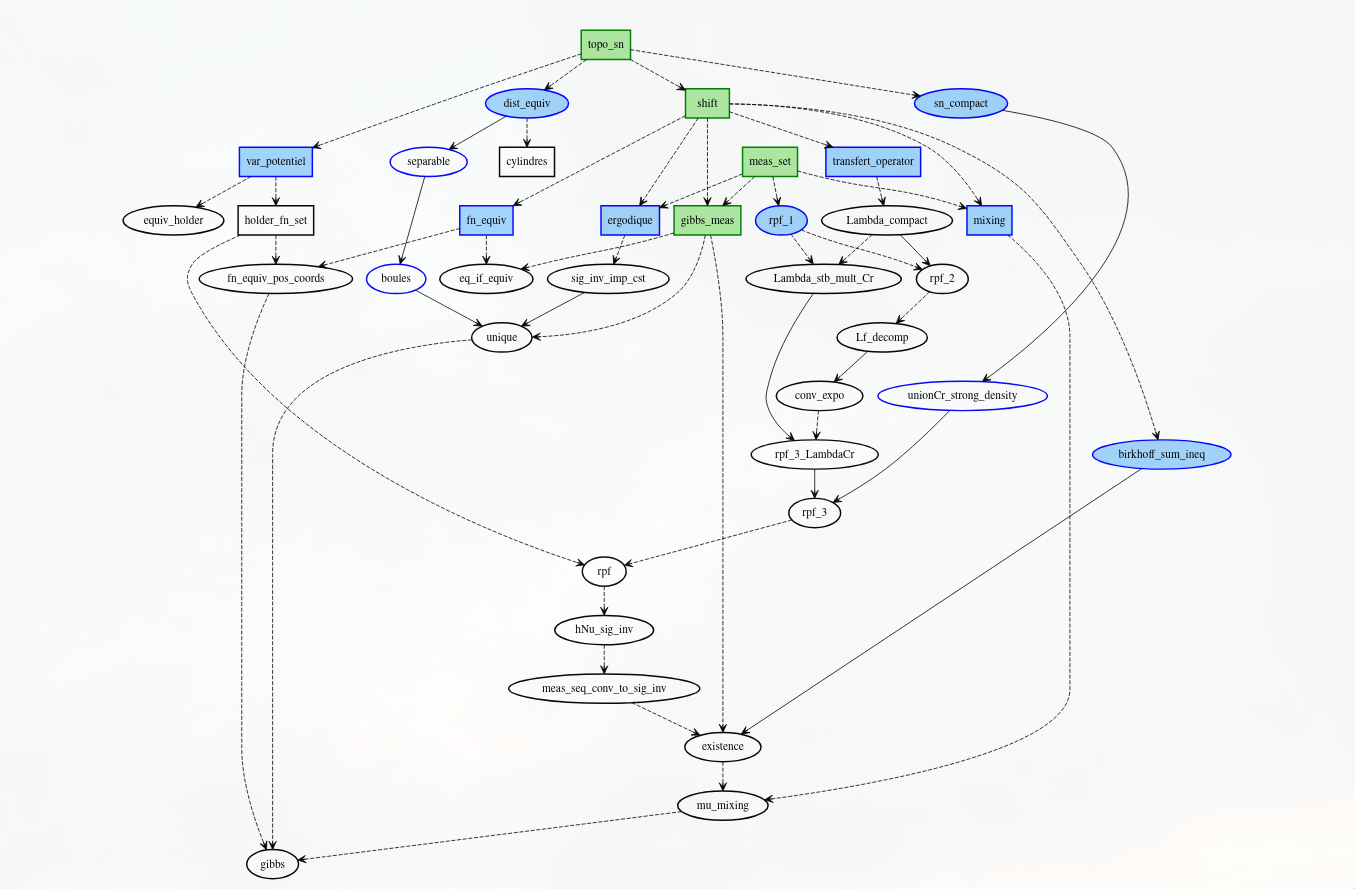
\includegraphics[width=.98\linewidth]{graph_1.png}
      \caption{État initial du graphe}
    \end{subfigure}
    \begin{subfigure}{.43\textwidth}
      \centering
      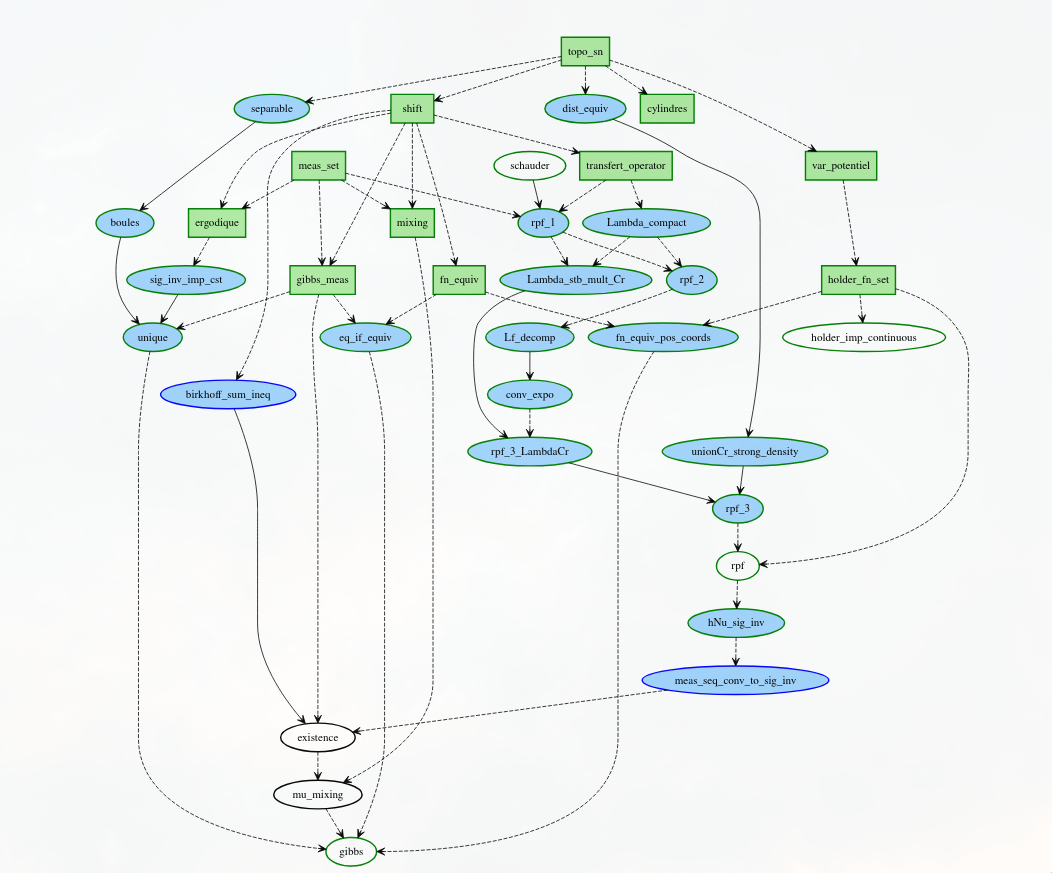
\includegraphics[width=.98\linewidth]{graph_8.png}
      \caption{État final du graphe}
    \end{subfigure}
  \end{figure}

  \begin{spacing}{0.8}
  {\scriptsize
  Les cases rectangulaires sont les définitions, les ellipses sont les lemmes, théorèmes, corollaires et propositions.
  Les couleurs en fond indiquent l'état d'avancement des preuves :
  le vert foncé pour pour les lemmes prouvés et dont les parents sont également prouvés,
  le vert clair pour les lemmes prouvés
  et le bleu pour les lemmes prêt à être prouvés (\textit{ie.} toutes les définitions nécessaires sont formalisés).
  Enfin les couleurs des bordures indiquent l'état d'avancement des énoncés des lemmes et des définitions :
  le vert pour les cases dont l'énoncé est formalisé
  et le bleu pour les cases dont l'énoncé n'est pas formalisé mais prêt à l'être.}
  \end{spacing}

  \subsection{Formalisation de l'énoncé du théorème}

  Dans un premier temps, j'ai donc converti chaque définition et résultat nécessaire pour le théorème de Bowen en code Lean
  afin de pouvoir écrire l'énoncé du théorème.
  Pour ce faire on a besoin notamment de définir la notion de mesure de Gibbs puis on peut alors énoncé le théorème
  avec le code suivant :
  \begin{figure}[ht]
    \centering
    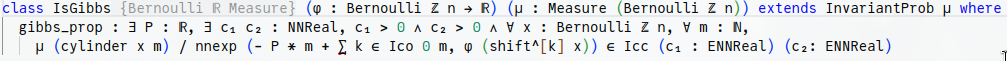
\includegraphics[width=\textwidth]{gibbs_def.png}

    \vspace{0.5cm}
    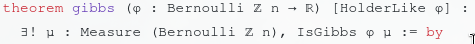
\includegraphics[width=0.6\textwidth]{gibbs_thm.png}
  \end{figure}

  Cependant, la preuve de ce résultat nécessite un certain nombre de lemmes intermédiaires qu'il faut également prouver
  et donc la preuve du théorème était trop longue par rapport au temps imparti.

  On a donc décidé de se concentrer sur la formalisation des énoncés et sur la preuve d'un lemme important
  de topologie des espaces ultramétriques, pour experimenter tout les aspects d'un assistant de preuves.

  Pour la formalisation des énoncés il a donc fallu dans un premier temps adapter le rapport de stage au format demandé
  par l'outil lean-blueprint, en ajoutant des détails et en décomposant certains énoncés pour correspondre davantage à la structure
  du code Lean. L'étape suivante était de traduire chaque définition et lemmes (sans les preuves) en un code le plus clair possible
  pour faciliter le travail d'écriture des preuves suivant l'ordre préconisé par le graphe de dépendance.
  Enfin, j'ai pu commencer à écrire des morceaux de preuves pour les lemmes les plus simples.
  Finalement au vu du nombre de preuve à convertir en code, il a fallu choisir un résultat dont la
  preuve était moins conséquente pour s'y consacrer.

  \subsection{Preuve d'un résultat topologique}

  Le choix qui a été fait était de prouver un théorème de topologie permettant de décomposer les ouverts d'un espace ultramétriques compact
  en une union disjointe de boules.
  Ce résultat était nécessaire pour réécrire la mesure des ouverts en somme de mesure de boules pour lesquelles on possède une estimation
  dans le cas des mesures de Gibbs.

  Afin de prouver ce résultat, la première étape était de réécrire de manière la plus détaillé possible sa preuve et d'en donner
  les étapes intermédiaires pour ensuite les convertir en lemme dans Lean pour pouvoir écrire les preuves de ces lemmes.
  L'étape finale à donc été d'écrire la preuve du théorème en utilisant tout les lemmes précédents.

  Cependant la traduction des preuves en Lean ne se fait pas littéralement, il faut souvent adapter les énoncés pour
  les faire correspondre aux lemmes déjà existants et prouvés dans Mathlib (la bibliothèque de Lean contenant une large variété de théorèmes).
  Ainsi, nous avons donc transformés l'énoncé mathématique standard, à savoir
  \begin{theorem*}
    Soit $\O$ un ouvert borné de $E$, alors il existe une partie $R \subseteq \O$ et une fonction $r : R \fun \R^*_+$ telle que
    $$\O = \bigsqcup_{x \in R}{B(x, r(x))}.$$
  \end{theorem*}
  en l'énoncé suivant, utilisant à la fois la théorie des types et des propriétés déjà présentes dans Mathlib :

  \begin{theorem*}
    Soit $\O$ un ouvert borné de $E$. Alors on a les propriétés suivantes :
    \begin{enumerate}
      \item $\bigcup_{s : S}{\Phi(s)} = \O$
      \item Si $s_1, s_2 : S$ sont distincts alors $\Phi(s_1)$ et $\Phi(s_2)$ sont disjoints.
    \end{enumerate}
    où $S$ est un type et $\Phi : S \fun B$ une fonction construites à partir de $\O$ et $B$ est le type des boules de $E$ incluses dans $\O$.
  \end{theorem*}

  On peut alors remarquer que les deux énoncés sont en fait équivalents, il s'agit simplement d'une reformulation
  plus maniable en Lean d'un même théorème, car elle fait intervenir des types et des fonctions largement utilisées dans Mathlib
  et qui sont donc plus faciles d'utilisation. Une fois converti en Lean, il peut s'écrire avec le code suivant :

  \begin{figure}[ht]
    \centering
    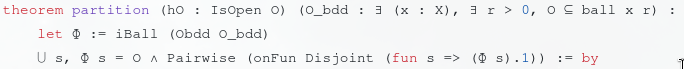
\includegraphics[width=0.8\textwidth]{topo_thm.png}
  \end{figure}

  Une preuve de ce théorème se trouve dans la section suivante et une formalisation de ce théorème est disponible ici (\textsc{Ajouter lien}).

\end{document}
